\begin{frame}[c]
  \tableofcontents[currentsection, hideothersubsections]
\end{frame}

\subsection{Slick}
\begin{frame}[c]
  \frametitle{Slick}
  \begin{block}{Caractéristiques}
    \begin{itemize}
    \item API de haut niveau java pour la conception de jeu en 2D;
    \item Basé sur l'API LWJGL librairie java reposant sur OpenGL.
    \end{itemize}
  \end{block}
  \begin{block}{Capacité de la librairie}
    \begin{itemize}
    \item Méthodes haut niveau pous la gestion d'un jeu;
    \item Gestion des images et des cartes facilités.
    \end{itemize}
  \end{block}
\end{frame}

\subsection{Map}
\begin{frame}[c]
  \frametitle{Tiled Map Editor}
  \begin{block}{Caractéristiques}
    \begin{itemize}
    \item Logiciel libre basé sur Qt (C++);
    \item Génération de cartes au format XML.
    \end{itemize}
  \end{block}
  \begin{block}{Utilisation dans notre cas}
    \begin{itemize}
    \item Multiplicité des cartes;
    \item Gestion de plusieurs couches par carte;
    \end{itemize}
  \end{block}
\end{frame}


\begin{frame}[c]
  \begin{figure}[htbp]
    \centering
    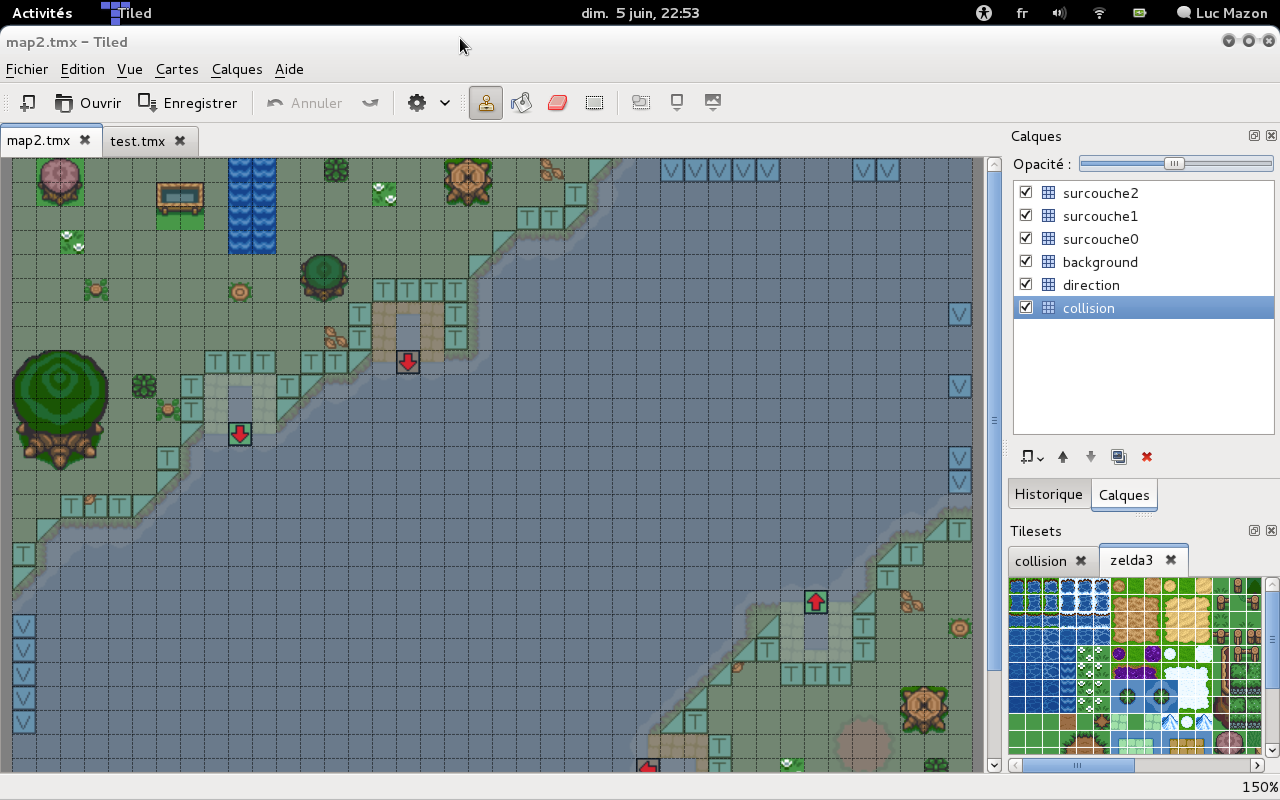
\includegraphics[width=0.8\textwidth]{images/tiled.png}
    \caption{Tiled Map Editor}
  \end{figure}
\end{frame}
